% ---------------------------------------------------------------------------- %
\chapter{The Linguometer}
\label{ch:linguometer}
%Simultaneous acquisition of phono-articulatory features
% ---------------------------------------------------------------------------- %
The CONTACT Project (NEST Contract No 5010) aims to investigate the
sensorimotor mechanisms common to both perception and production of speech and
manipulation.

Infants develop motor and language abilities in
parallel~\citep{lennenberg:1967,kandel.schwartz.jessel:2000} 
and the results of the studies presented in the previous Chapters support the
hypothesis that there is a functional connection between language related and
motor-control related areas in the dominant left
hemisphere, where Broca's areas is located~\citep{fadiga.etal:PRESS}. 
The last decade of neurophysiological studies focused on the novel idea that
actions are represented in terms of goals rather then in terms of
procedures.
In fact, single unit recordings of monkey F5 neurons demonstrate that a subset
of cells discharge both during the execution of goal-directed transitive 
actions and during the observation of a similar action, thus linking production
to perception~\citep{rizzolatti.etal:1996}.
%As~\citet{rizzolatti.arbib:1998} initially suggested, Broca's area in humans 
%could have evolved from area F5 in monkeys where hand and mouth movements are
%represented, and where the mirror system is located. 
As~\citet{rizzolatti.arbib:1998} initially suggested, Broca's area in humans 
and area F5 in monkeys could have evolved from a common ancestor region.
Evidence for a mirror system in humans is provided by brain imaging 
experiments, as discussed in other deliverables.
%and the results of a part of those experiments have been discussed in
%Section~\ref{sec:actions:human}.

According to the motor theory of speech perception, the real objects of speech
are the speaker intended gestures, represented in the brain as invariant motor 
commands~\citep{liberman.mattingly:1985}.
Moreover, the sender and the receiver of a message must share a common
repertoire of speech motor actions. 
This motor vocabulary must be embedded in a unique ``module'' that is involved
both in production and perception tasks.
The mirror system appears as a good candidate for this role.

The topics discussed in the previous Chapters, here briefly presented, provide
sufficient clues for a unifying theory of mechanisms underlying
manipulation and speech, notwithstanding the obvious differences between the
effectors and sensory modalities
involved~\footnote{CONTACT Annex I - ``Description of Work'', March 2005}.

A question that still remains open concerns the development of language
and manipulatory skills in ``social infants''.
Are those processes fundamentally linked or is it just a case that they develop
in parallel going through a well-known sequence of 
stages that appear common to all cultures and all
languages~\citep{lennenberg:1967}?

The CONTACT Project is investigating the parallel development of manipulatory
and language-oriented skills from a multidisciplinary perspective, involving
roboticians, neuropsychologists and child-development experts.
The scientific results of the project will be validated on an embodied artifact,
a humanoid robot, that will develop its own capabilities in both manipulation
and language.
The remaining Chapters of this thesis illustrate the work done for the CONTACT
Project assembling and running an experimental setup for the simultaneous 
acquisition of phono-articulatory features, the ``Linguometer''.
The data recorded with the Linguometer will be used to build an audio-motor map 
that will allow the robot to recognize at least a small subset of words.
If the hypothesis that speech relies on invariant motor commands is correct, 
the articulatory features recorded with the Linguometer should allow the
model to outperform similar models based only on the phonetic features.
The performance of the model will be tested in two cases.
In the first case training and testing will be done using just phonetic
features. In the second case, both phonetic and articulatory (motor) features
will be used during training, while testing will still rely on just the acoustic
features.
The idea is to build an audio-motor map (AMM), that will translate the acoustic 
features to motor features. 
%The motor space, that is the kinesthetic representation of speech, should be
%simpler than the corresponding phonetic space (less degrees of freedom, is it
%correct Paul?) and, according to Liberman's theoretical framework and the
%studies on the mirror system, should be characterized by some degree of
%invariance (again, does it make sense?).
The motor space, that is the kinesthetic representation of speech, constitutes
a better space in which to perform learning and classification.
In fact, according to Liberman's theoretical framework and the
studies on the mirror system, the motor representation of speech should be 
characterized by some degree of invariance.

\citet{metta.etal:2006} developed a biologically-inspired Bayesian model of
the mirror system.
The authors demonstrated that kinesthetic and tactile information associated to
a certain hand action can simplify the recognition of the same action when the
only information available is the visual one.
Moreover, the experimenters were interested in determining if the artificial
model
of the mirror system was effectively able to learn the motor invariance common
to different grasping types.
In order to feed the appropriate kinesthetic information to the system, a data
glove (CyberGlove by Immersion) with 22 sensors.
A magnetic tracker recorded the position and the orientation of the hand with
respect to a reference frame.
Tactile features were provided by two touch sensors. The actions performed by
the subjects were recorded using a pair of CCD cameras, thus providing the
visual information required by the visuomotor model. 
The six recorded subjects were asked to grasp three different objects 
(e.g.: a small glass ball, a rectangular solid, and a large sphere) making three
different grasping actions (e.g.: precision grasping, power grasp and power
grasp).
The visual features of the grasping actions were recorded from 12 different
locations. Moreover, each action was performed 5 times.
Once the data was recorded using the setup here described, the model was
trained and tested in two cases. Classification rate of the perceived actions is
used to describe the performance of the model.
In the first case, the model was trained and tested only using visual
features.
In the latter, the model was trained using all the available visuo-motor 
features and tested by feeding to the system only the visual
information.
The authors report a classification rate of $97\%$ (training set) and $80\%$
(test set) for the first case. 
When the model was fed using visuo-motor features during training, its
performance was higher in the test set ($98\%$ training set, $97\%$ test 
set), demonstrating that, at least in the case of the described model, the
motor information plays a crucial role in the action recognition process.
%In fact, when available, the visuo-motor features were used to build a
%more accurate visuo-motor inverse model (or VMM, visuo-motor inverse map)
%than in the plain visual case.
In fact, when available, the visuo-motor features were used to build a
visuo-motor map (VMM) that mapped the visual features onto the motor space.

Measuring the activity of the articulators (the tongue, the larynx, the lips and
the jaw) during speech is not trivial. 
Firstly, the articulators are fairly inaccessible.
Secondly, no Linguometer-like instrumentation is available on the market.
Lastly, speech production should not be affected by the recording devices.
Taking these three points into account, the Linguometer has been assembled 
interconnecting different instruments, building custom devices, and finally
writing the required software (e.g.: setup-control, stimuli presentation, data
handling, data processing, signal synchronization and segmentation).
Once the Linguometer was finally been built, a total of nine
experiments have been run (Chapter~\ref{ch:experiments}) and the data has been
processed (Chapter~\ref{ch:results}).\\

This Chapter describes how the Linguometer has been built, using a bottom-up
approach. 
Firstly, the instrumentation on which the Linguometer is based is briefly
described, in terms of both principles and implementation
(Section~\ref{ch:linguometer:instrumentation}).
(to be continued). 
% ---------------------------------------------------------------------------- %
\section{Instrumentation}
\label{ch:linguometer:instrumentation}
% ---------------------------------------------------------------------------- %
The Linguometer consists of ``a constellation of hardware and
software''\footnote{CONTACT Annex I - ``Description of Work'',
March 2005} that allows the simultaneous recording of acoustic and articulatory
data.
It is made up of several interconnected devices; some of those are 
synchronized in hardware, while the remaining rely on post-processing
synchronization.
The devices and the recording room were made available by the CRIL 
laboratory\footnote{CRIL: Centro di Ricerca Interdisciplinare sul Linguaggio 
(Interdisciplinary Language Research Center).
Homepage: http://www.cril.unile.it.},
where the Linguometer has been built during the period that spans
from August 2006 to January 2007.\\
This Chapter aims to describe how the instrumentation works and why it is
important for the recordings required by the CONTACT Project.
%Few technical issues are presented here, the building blocks the
%Linguometer relies on are better discussed in
%Section~\ref{ch:linguometer:architecture}.
Firstly the author describes the recording devices that characterize the
Linguometer (Section~\ref{ch:linguometer:instrumentation}).
Secondly, the Linguometer's architecture is discussed, mainly focusing onto the
synchronization topic (Section~\ref{ch:linguometer:architecture}).
Lastly, the author presents and discusses few technical issues emerged during
the integration process (Section~\ref{ch:linguometer:technical}).
% ---------------------------------------------------------------------------- %
\subsection{Electromagnetic articulograph}
\label{sec:linguometer:instrumentation:ag}
% ---------------------------------------------------------------------------- %
An electromagnetic articulograph (EMA) was used to track the movements of a set
of sensors glued on the tongue, on the lips, on the front teeth and on 
a pair of glasses, as it is shown in Figure~\ref{fig:experiments:map}.
%(for head-movement compensation).
The pictures in Figure~\ref{fig:linguometer:ag:tongue} show how the sensors are
positioned onto the tongue to track tongue movements during speech production.
The device used for the Linguometer is an ``Articulograph AG500'' made by
Carstens Medizinelektronik GmbH, G\"ottingen, Germany.

The AG500 articulograph could determine the three-dimensional spatial 
arrangement (Cartesian coordinates $x$, $y$ and $z$) and the orientation
(spherical coordinates azimuth $\theta$ and elevation $\rho$)
of up to twelve 
directionally sensitive magnetic field sensors at a sampling frequency of 200Hz.
The measuring sensors are single axis coils.
Six reference coils, arranged to form a three-dimensional frame of
reference, emit six magnetic fields at different frequencies:
7500, 8750, 10000, 11250, 12500 and 13750 Hz.
The alternating current induced in the sensor by the alternating magnetic fiels
of the reference coils is measured.
The measuring device distinguishes and separates the alternating voltages
induced by the individual alternating magnetic fields by their 
frequencies.
During a recording session the separated and digitized current signals are
sent in real-time to the AG500 control PC (using an Ethernet connection).
Software provided by Carstens Medizinelektronik GmbH stores the current values
on the hard drive of the control PC, making those available for the spatial 
arrangement determination process.
The main idea behind the spatial determination process is that the distance 
between the sensors and the reference coils is determined from the
absolute values of the induced currents. 
The position vector and the direction vector of a sensor can then be calculated
starting from the six field equations of the reference coils, using an iterative
method~\citep{zierdt.carstens:1993}.

% ---------------------------------------------------------------------------- %
\begin{figure}
	\centering
	  \subfigure[\label{fig:linguometer:ag:intro:cube1}]
		{\includegraphics[width=0.45\textwidth]{include/linguometer/images/ag_cube1.tps}}
		\hspace{0.05\textwidth}
	  \subfigure[\label{fig:linguometer:ag:intro:cube2}]
		{\includegraphics[width=0.45\textwidth]{include/linguometer/images/ag_cube2.tps}}

	\subfigure[\label{fig:linguometer:ag:intro:magazine}]
		{\includegraphics[width=0.45\textwidth]{include/linguometer/images/ag_magazine.tps}}
		\hspace{0.05\textwidth}
	\subfigure[\label{fig:linguometer:ag:intro:circal}]
		{\includegraphics[width=0.45\textwidth]{include/linguometer/images/ag_circal.tps}}

	\caption[Articulograph AG500]{\textbf{Articulograph AG500: EMA-Cube, magazines and Circal}:
	(a) Prof. M. Grimaldi, CRIL evaluates the correct posture required by the
	subjects when recording using the articulograph AG500.
	Five out of the six reference coils are visible: two red, two green and a
	blue one. The sixth sensor (blue) is located just behind Prof. Grimaldi's
	head, on the top of the EMA-Cube.
	Just at the top of Prof. M. Grimaldi's head, the Circal mounting slot is
	visible (white structure).
	(b) Prof. M. Grimaldi during an experiment (some sensor wires are visible).
	(c) A magazine with four sensors mounted. 
	(d) The magazine attached to the Circal calibration device.
	Photos courtesy of Prof. M. Grimaldi and Dr. B. Gili Fivela, CRIL.}
	\label{fig:linguometer:ag:intro}
\end{figure}
% ---------------------------------------------------------------------------- %

The AG500 articulograph is sensitive to electrically or magnetically conductive
objects. 
In fact, if one or more of those objects are placed nearby the transmitter (or
reference) coils, the generated magnetic fields are distorted.
If the interfering object moves, a time-varying distortion affects the
magnetic field.
On the other hand, if the interfering object does not move, the
distortion is constant in time (static distortion). 
Furthermore, in the second case, the interference can be
corrected since the resulting error depends on the distance between the
reference coils and the conductive object.

Before each recording session, the AG500 is calibrated in order to
tune the six field equations that map current values to position/orientation
values.
Furthermore, calibration is useful to compensate for the possible static
distortions. 
The twelve sensors (or less, it depends on how many sensors the investigation 
requires) are placed in appropriate magazines mounted on a dish (Circal) inside
the  frame of reference (EMA-Cube).
Figure~\ref{fig:linguometer:ag:intro} shows the previously mentioned devices.
A program developed by Carstens Medizinelektronik GmbH rotates the Circal using an
electrical motor (located on top of the EMA-Cube) moving each sensor until it 
reaches a well known position.
Once the target position is reached, the corresponding current amplitudes  
are acquired. The control PC then calculates the calibration factors that are
necessary to convert the currents acquired during an
investigation in consistent positions.
A synchronization device (Sybox Opto-4) is connected to the articulograph
AG500 and
%This device is used by the Linguometer to allow the synchronized acquisition of
%phono-articulatory gestures.
it is heavily used by the Linguometer in order to allow the synchronized 
acquisition of phono-articulatory gestures.
For this reason, a few words should be spent describing how this device works.

Both the Sybox Opto-4 device and a microphone are connected to the Line-In jack
of the control PC sound card (left and right channel respectively).
After an investigation is started, the recording software asks the AG500 to
start sending data and waits for the synchronization signal to appear on the
left-channel of the Line-In connector.
When the synchronization signal is detected, the acquisition software starts
recording both the speech data and the amplitudes data.
A ``low enough'' delay affects the synchronized signals, although its value is
unpredictable and not constant (Bahne Cartsens, personal  communication. 
November 2006).
Cartsens Medizinelektronik GmbH does not provide the source code of the AG500
software (although the Sybox-Opto4 schematic is available).
For this reason, it has not been possible to measure or to estimate the delay
affecting the synchronization, and it will be considered negligible from now on.

% ---------------------------------------------------------------------------- %
\begin{figure}
	\centering
	  \subfigure[\label{fig:linguometer:ag:tongue:f}]
		{\includegraphics[width=0.45\textwidth]{include/linguometer/images/ag_tongue_f.tps}}
		\hspace{0.05\textwidth}
	  \subfigure[\label{fig:linguometer:ag:tongue:m}]
		{\includegraphics[width=0.45\textwidth]{include/linguometer/images/ag_tongue_m.tps}}

	\caption[Articulograph sensors glued on the tongue]{\textbf{Articulograph sensors glued on the tongue}:
	(a) A female subject and (b) a male subject with dorsal and coronal articulograph
	AG500 sensors glued on the tongue. The female subject also has sensors glued
	on the lips and on the upper and lower incisive teeth.
	The reader may find Figure~\ref{fig:experiments:map} useful to better
	understand how the sensors are positioned.}
	\label{fig:linguometer:ag:tongue}
\end{figure}
% ---------------------------------------------------------------------------- %

Once the amplitudes have been recorded, positions can be calculated using the
Cartsens Medizinelektronik GmbH software or the open source TAPADM ToolBox by A.
Zeirdt\footnote{TAPADM homepage:
http://www.phonetik.uni-muenchen.de/\~{}andi/EMAPage/}.
Furthermore, since the subject's head is not constraint during the
investigation, three sensors are used to track head movement and then to
compensate for it.
Moreover, the sensors do need to be kept close to the geometrical center of the
frame of reference.
%center of mass. 
Particularly, Carstens Medizinelektronik GmbH recommends to keep the sensors
inside the 15 cm diameter spherical volume that shares its geometrical center 
with the geometrical center of the frame of reference.
% ---------------------------------------------------------------------------- %
\subsection{Ultrasound system}
\label{sec:linguometer:instrumentation:us}
% ---------------------------------------------------------------------------- %
Modulating the shape of the vocal tract, the tongue plays a critical role in
articulation.
Being positioned deep in the oral cavity, the tongue is a fairly inaccessible 
articulator and requires measuring devices to be inserted inside the mouth. 
Tongue recording for the CONTACT Project took place by gluing a few AG500
sensors on
the tongue and recording tongue motion on the sagittal plane using the Toshiba
Aplio XV Ultrasound System provided with a low frequency convex transducer by
Toshiba, positioned submentally.
Ultrasound investigation of the tongue motion is both non-invasive and non
obtrusive, thus non affecting speech production.
Furthermore, ultrasound images provide the full profile of the tongue
dorsum, although the apex and the radix are often occluded during speech
production
by the jaw and by the hyoid bone respectively. 
According to~\citet{stone:2005}, the acoustic shadows of the hyoid bone can be
used to detect swallowing events.
On the other hand, generally no more than 1 cm of the tongue apex is obscured
by the jaw shadow.

Medical sonography uses high frequency (2-14 MHz) sound waves emitted from a
piezoelectric crystal that produces an image by using the reflective properties
of sound waves.
Piezoelectric crystals undergo a change in size when a voltage is applied.
If the voltage is alternating, the crystal oscillate at high frequency,
producing high frequency sound waves.
Piezoelectric crystals can also be used as ultrasound waves detectors. 
In fact, if a force is applied to a crystal, it generates a voltage.
The ultrasound transducer is equipped with a mono-dimensional array of
piezoelectric transducers, multiplexed in time so that only one crystal emits
sound waves in a given time interval. Immediately after the crystal emits the
pressure wave, all the remaining crystals are used to convert the received 
echoes to voltage values. Voltage values are then processed and the image
is reconstructed.
In order to generate pressure waves, the crystals are heated at high 
temperature so that the molecules they are made of are magnetically aligned  
by the means of dipolar molecular alignment.
When a voltage is applied to the crystals, the molecules first twist in one
direction increasing the crystals' thickness, then in the reverse direction
thus decreasing the thickness~\citep{stone:2005}.
If the applied voltage is alternating, this change in 
thickness produces cyclic sound pressure waves.
The thickness of the crystals determine the resonant frequency of the crystals
themselves.
Moreover, the higher the resonant frequency is, the shorter the wavelength is,
and short wavelengths are important to increase the spatial resolution of the
transducer (\emph{ibid}).

% ---------------------------------------------------------------------------- %
\begin{figure}
	\centering
	  \subfigure[\label{fig:linguometer:us:constraints:f}]
		{\includegraphics[width=0.45\textwidth]{include/linguometer/images/us_larynx_f.tps}}
		\hspace{0.05\textwidth}
	  \subfigure[\label{fig:linguometer:us:constraints:m}]
		{\includegraphics[width=0.45\textwidth]{include/linguometer/images/us_larynx_m.tps}}

	\caption[Ultrasound transducer constraints]{\textbf{Ultrasound transducer constraints}:
	(a) A female subject and (b) a male subject during linguometer recordings.
	The ultrasound probe is placed submentally. The black strap hold the
	laryngograph sensors in fixed position.
	In the specific case of the male subject, the ultrasound transducer touches
	the larynx.}
	\label{fig:linguometer:us:constraints}
\end{figure}
% ---------------------------------------------------------------------------- %

When an ultrasound wave reaches an interface between materials with different
impedance properties, it is reflected. Large density gradients create a strong
echo (e.g.: tissue/air and tissue/bone interfaces) while low density gradients
bring to weak echoes (e.g.: tissue/water and tissue/tissue interfaces).
Figure~\ref{fig:linguometer:us:frame} shows a frame grabbed from an ultrasound
investigation of tongue motion.
The brightest area in the image is the subject's tongue. The brighter the
pixel is, the higher the density gradient is, thus the acquired echoes.
Tongue lamina is clearly visible since a great density gradient exists between
the muscle tissue/air interface.
The same happens for the lower tongue surface.
The hard palate, the hyoid bone and the jaw are not visible since they adsorb
the sound waves, and thus do not produce echoes. 
At the beginning of this Section, it has been said that the tongue and the
palate play a critical role in articulation, since the they modulate the shape
of the vocal tract.
Due to the facts here described, acquiring the palate's profile during the
experiments is not possible, and for this reason the subjects' palates were
recorded off-line, as better discussed in
Section~\ref{sec:experiments:recording}.

While experimenting with tongue recordings, it appeared clear that not all
tongues are suitable for ultrasound investigation during speech production 
tasks.
Furthermore, similar and more detailed conclusions are reported
by~\citet{stone:2005}.
Firstly, female subjects appear to be better candidates for speech production
investigation. Women often image better than men, probably because the tongues
of men are thicker and fatter (fat tissue scatters sound).
Furthermore, men do have a bigger larynx that protrudes from the neck. This
anatomical difference plays a crucial role in speech production recordings,
because the ultrasound transducer is placed submentally and when the larynx
moves, it touches the transducer. 
This mechanical contact produces pain and higher swallowing rates in the
male subjects and made male recordings with the Linguometer quite impractical 
(Fig.~\ref{fig:linguometer:us:constraints}).
Female subjects also have smoother tongues thus producing higher-quality
gradients in the image.
Furthermore, subjects with high salivation often provide better results.
According to~\citet{stone:2005}, the saliva forms a thin film around the tongue,
thus becoming smoother and acting as a better reflector.
Although high salivation provides better ultrasound images, the large amount of
saliva easily wears out the glue used to attach the articulograph sensors to the
tongue. For this reason, subjects with high salivation were not
recorded~(Chapter~\ref{ch:experiments}).

% ---------------------------------------------------------------------------- %
\begin{figure}
	\centering
	  \subfigure[\label{fig:linguometer:us:intro:full}]
		{\includegraphics[width=0.45\textwidth]{include/linguometer/images/us_full.tps}}
		\hspace{0.05\textwidth}
	  \subfigure[\label{fig:linguometer:us:intro:probe}]
		{\includegraphics[width=0.45\textwidth]{include/linguometer/images/us_probe.tps}}

	\caption[Ultrasound System Toshiba Aplio XV]{\textbf{Ultrasound System Toshiba Aplio XV}:
	(a) The Toshiba Aplio XV Ultrasound System. (b) The convex transducer used for the 
	recordings.}
	\label{fig:linguometer:us:intro}
\end{figure}
% ---------------------------------------------------------------------------- %

Figure~\ref{fig:linguometer:us:intro:full} shows the Toshiba Aplio XV ultrasound
system while~\ref{fig:linguometer:us:intro:probe} shows the convex transducer 
used for the Linguometer recordings.
Figure~\ref{fig:linguometer:us:frame} shows a frame grabbed from the
Toshiba Aplio XV system using an acquisition card attached to the S-Video
Aplio XV video output.
The Toshiba Aplio XV system was shipped with a RAW frame acquisition plug-in
that
allows us to acquire a maximum of 5 seconds of RAW frames, independently from
the acquisition frame rate and the frame resolution.
A RAW frame is intended to be the reconstructed tongue image without any
processing applied.
The acquired sequences are temporarily accumulated in a hardware buffer until
the maximum capacity of the buffer is reached. 
Once it is full, the buffer needs to be emptied saving the RAW data on the 
Aplio XV internal hard drive, shared on the network via the SMB/CIFS network
protocol\footnote{SMB/CIFS: Microsoft standard resource exchange protocol.}.

The RAW plug-in was initially designed by Toshiba for heart investigations, and
for this reason the maximum length of a RAW acquisition was limited to 5
seconds,
probably enough for heart disease studies.
%Moreover, the plug-in did require an experimenter to be used since no automated
%recording procedure is implemented in the plug-in itself.
Moreover, using the plug-in is laborious and time-consuming since no automated 
recording procedure is implemented in the plug-in itself, thus an experimenter
is required to handle the RAW recordings.
For those reasons, the RAW plug-in was dropped, and the S-Video output was
recorded. 
% ---------------------------------------------------------------------------- %
\begin{figure}[htbp]
	\centering
	\epsfig{file=include/linguometer/images/us_frame.tps, width=0.65\textwidth}
	\caption[Ultrasound System video frame]{\textbf{Ultrasound System video frame}:
	A frame grabbed from the S-Video connector. It shows the tongue (resting
	position) of a 25
	years old female subject and the tongue recording convention used for the
	linguometer (sagittal plane, apex on the right, dorsum on the top).}
	\label{fig:linguometer:us:frame}
\end{figure}
% ---------------------------------------------------------------------------- %

Surely the S-Video output does not ensure an image quality comparable with the
RAW data image quality, but consistently simplifies the recording work flow.
A non trivial problem arises recording the S-Video stream. In fact, the 
Toshiba Aplio XV system is a closed source device intended for clinical use 
and probably the image reconstruction does not happen in real-time. 
Toshiba Medical System Europe did not provide enough details about the
processing the reconstructed frames undergo before visualization on the monitor
or presentation on the S-Video connector. 
Frame persistence\footnote{Frame persistence: a technique used to enhance the
quality of a video stream by averaging each frame with few surrounding ones.} 
and many other filters have been disabled in
order to record frames ``corrupted'' by the smallest possible amount of 
post-processing operations.
Moreover, no details were provided about the delays characteristic of the Aplio
XV system.
%All those issues are discussed in Chapter REF HERE.
% ---------------------------------------------------------------------------- %
\subsection{Laryngograph}
\label{ch:linguometer:instrumentation:lg}
% ---------------------------------------------------------------------------- %
Electroglottography is a technique used to register laryngeal behavior measuring
the change in electrical impedance across the throat during speech production.
The EGG device used for the Linguometer is a ``Laryngograph Microprocessor`` by
Laryngograph Ltd, London, United Kingdom. 
% ---------------------------------------------------------------------------- %
\begin{figure}
	\centering
	  \subfigure[\label{fig:linguometer:lg:intro:front}]
		{\includegraphics[width=0.45\textwidth]{include/linguometer/images/lg_front.tps}}
	  \hspace{0.05\textwidth}
	  \subfigure[\label{fig:linguometer:lg:intro:rear}]
		{\includegraphics[width=0.45\textwidth]{include/linguometer/images/lg_rear.tps}}
	  
	  \subfigure[\label{fig:linguometer:lg:intro:sensors}]
		{\includegraphics[width=0.45\textwidth]{include/linguometer/images/lg_sensors.tps}}
	  \hspace{0.05\textwidth}
	  \subfigure[\label{fig:linguometer:lg:intro:strap}]
		{\includegraphics[width=0.45\textwidth]{include/linguometer/images/lg_strap.tps}}

	\caption[Laryngograph MicroProcessor]{\textbf{Laryngograph MicroProcessor}:
	Front (a) and rear (b) view of the Laryngograph MicroProcessor. The USB
	connector, the microphone and the EGG electrodes connectors are
	shown. (c) EGG electrodes, available in three different sizes. (d) A subject
	wears the EGG electrodes, kept in fixed position using the visible black
	flexible band.
	Photos (a), (b) and (c) courtesy of Prof. M. Grimaldi and Phd. B. Gili Fivela, CRIL.}
	\label{fig:linguometer:lg:intro}
\end{figure}
% ---------------------------------------------------------------------------- %


An high frequency current, small both in voltage and amperage, passes between
two electrodes situated at the surface of the throat at the level of the 
thyroid cartilage. The sensors are shown in 
Fig.\ref{fig:linguometer:lg:intro:sensors} while the correct positioning onto
the subjects' neck is shown in Fig.\ref{fig:linguometer:lg:intro:strap}.
The electrodes, kept in fixed position by an elastic band, are made of copper
and their area ranges from 3 to 9 cm$^{2}$.
An alternated current generator supplies an high frequency (usually from 300 kHz
to 5 MHz) sinusoidal current to the electrodes. The current amplitude is in the
oder of few milliamperes while the applied voltage is around 0.5 V.
When the vocal folds move, a rapid variation of the conductance is observed in
the EGG signal applied across the larynx.
The percentage of amplitude modulation reflects the percentage change in the
path followed by the applied current. 
The observed impedance is least for full vocal folds contact because there are 
many parallel equally conductive paths between the electrodes.
Furthermore, the combined total parallel resistance is less than the resistance
of any one path. 
For those reasons, the tissue impedance seen by the EGG device is inversely
proportional to the lateral contact area of the vocal 
folds~\citep{childers.krishnamurthy:1985}.

% ---------------------------------------------------------------------------- %
\begin{figure}[htbp]
	\centering
	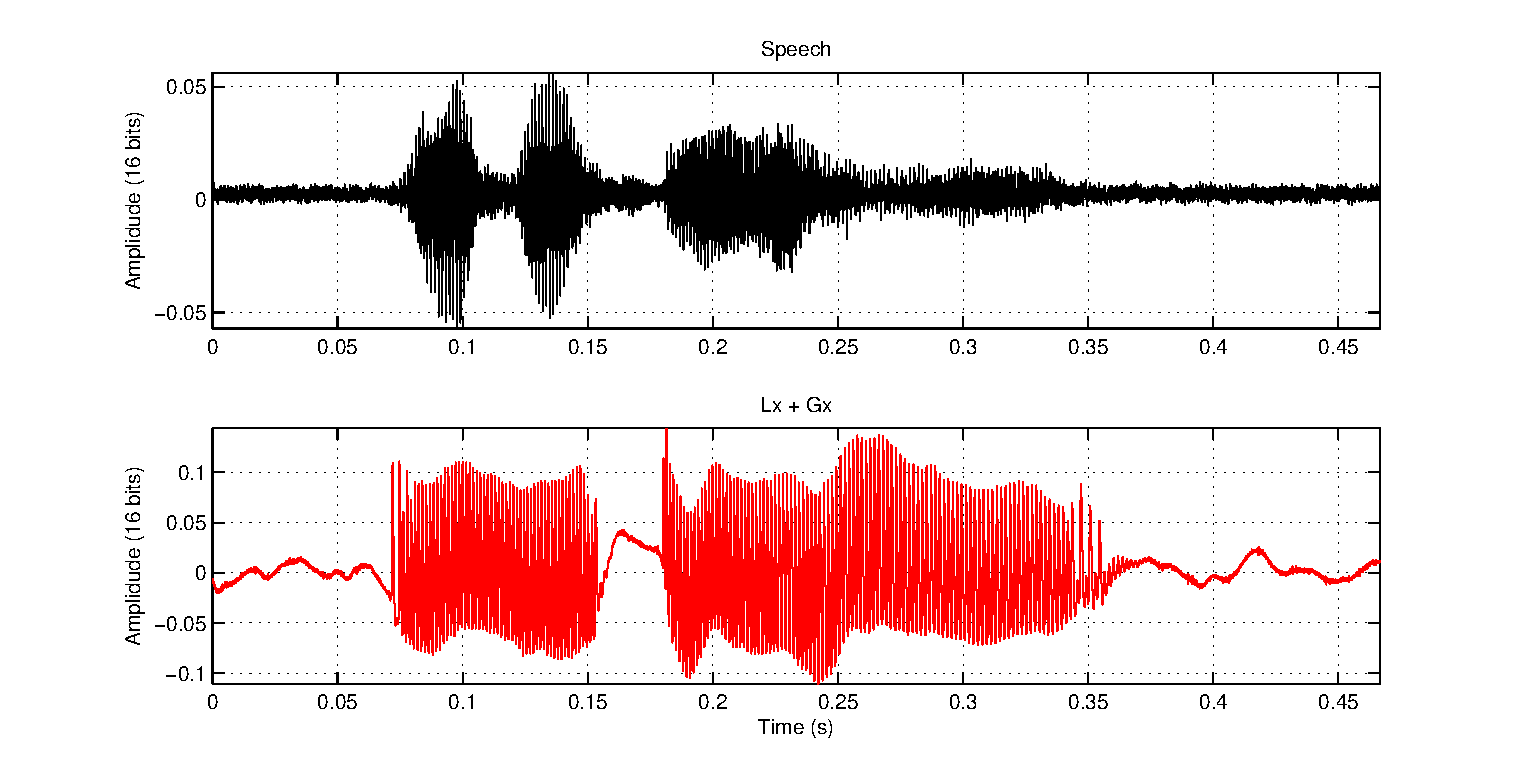
\epsfig{file=include/linguometer/images/lg_example.eps, width=1.00\textwidth}
	\caption[Laryngograph signals]{\textbf{Laryngograph signals}: speech signal 
	(on the top) and EGG signal (on the bottom) acquired with the Laryngograph
	Microprocessor by Laryngograph Ltd.
	The signals were acquired from a 27 years old female subject saying the
	Italian word /lavatoio/ (/sink/ in English).
	The sampling frequency is 16 kHz for both signals.
	The low-frequency component of the EGG signal (Gx signal) is clearly visible 
	before the onset and after the utterance. 
	}
	\label{fig:linguometer:lg:example}
\end{figure}
% ---------------------------------------------------------------------------- %

The amplitude of the EGG signal depends on many factors such as the
positioning of the electrodes, the amount of fat and muscles tissue in the 
subjects neck, the impedance of the skin, the position of the 
larynx and the and shape of the surrounding cartilages.
The EEG signal is made up by two different components. The first one depends on
the vibrational movement of the vocal folds, and is referred as the 
\emph{Lx} signal. 
The latter one is due the slower movement of other structures (e.g.: vertical
movements of the larynx characterize swallowing) and it is referred as the
\emph{Gx} component. The Gx signal could be easily filtered since its frequency
is much lower than the frequency of the Lx signal.

The Laryngograph Microprocessor device records both the EGG signal and the
speech signal synchronously. The device is attached to a control PC using a
standard USB interface. Laryngograph Ltd provides the software that handles the
signal recording.
Both the EGG signal and the speech signal are acquired at 16 kHz. 
Figure~\ref{fig:linguometer:lg:example} shows an example of the synchronized
speech and EGG signals.
% ---------------------------------------------------------------------------- %
\subsection{Audio and video devices}
\label{ch:linguometer:instrumentation:av}
% ---------------------------------------------------------------------------- %
In order to acquire the speech signal, two microphones were used.
The first microphone, a Shure SM7B, recorded the speech signal successively
routed to the articulograph AG500 PC.
A second microphone, a Shure SM58, was directly attached to the EGG device
by Laryngograph Ltd.
% ---------------------------------------------------------------------------- %
\begin{figure}
	\centering
	  \subfigure[\label{fig:linguometer:av:intro:mics}]
		{\includegraphics[width=0.45\textwidth]{include/linguometer/images/av_mics.tps}}
		\hspace{0.05\textwidth}
	  \subfigure[\label{fig:linguometer:av:intro:mixer}]
		{\includegraphics[width=0.45\textwidth]{include/linguometer/images/av_mixer.tps}}

	  \subfigure[\label{fig:linguometer:av:intro:camera}]
		{\includegraphics[width=0.45\textwidth]{include/linguometer/images/av_camera.tps}}
		\hspace{0.05\textwidth}
	  \subfigure[\label{fig:linguometer:av:intro:dv}]
		{\includegraphics[width=0.45\textwidth]{include/linguometer/images/av_dv.tps}}

	\caption[Audio/Video acquisition devices]{\textbf{Audio/Video acquisition devices}:
	(a) The microphones used during the recordings are placed one closed to the
	other. (b) The mixer mixes and controls the gain of the
	Audio/Synchronization signals and routes the final signal to other devices
	used for the linguometer.
	(c) The DV camcorder used for facial
	expression acquisition is flipped 90 degrees on	its side in oder to have a
	better resolution of the face.
	(d) Terratec CameoConvert Audio/Video acquisition card.}
	\label{fig:linguometer:av:intro}
\end{figure}
% ---------------------------------------------------------------------------- %

A Behringher Xenyx 802 Mixer was used to mix speech ans synchronization signals.
A Terratec CameoConvert audio/video acquisition card was used to acquire the
ultrasound system S-Video stream, the speech and the synchronization signals.
Finally, a Canon MV960 DV camcorder was used to record facial expressions. 
Figure~\ref{fig:linguometer:av:intro} shows the previously cited devices.
The connections between those instruments and few technical issues are discussed
in Sections~\ref{ch:linguometer:architecture}
and~\ref{ch:linguometer:technical}.
% ---------------------------------------------------------------------------- %
\subsection{Recording support devices}
\label{ch:linguometer:instrumentation:custom}
% ---------------------------------------------------------------------------- %
As already explained, the main goal reached with the Linguometer pertains to the
simultaneous acquisition, using the instrumentation previously described, of
a wide set of phono-articulatory features.
The instrumentation used for the Linguometer was not designed for parallel
recording, albeit the Cartsens GmbH AG500 articulograph was shipped with a
synchronization devices suitable for synchronizing a maximum of three
other devices.
A total of three custom devices, here described, have been designed and built.
%The motivation that brought to the building process better described 
%in Chapter REF HERE.

The first device that has been built is an ultrasound transducer stand.
As discussed at the beginning of the Chapter, the articulograph AG500 plays a
crucial role in the design of the Linguometer. 
In fact, it allows to track up to twelve sensors at very high frequency (200Hz),
thus allowing to detect very fast movements of the
articulators~(Section~\ref{sec:linguometer:instrumentation:ag}).
On the other hand, the articulograph provides low spatial resolution recordings
of the tongue.
In the particular case of the experiments run with the Linguometer, a total of 
five sensors were placed on the tongue, three sagittally and two coronally.
To avoid this limitation in spatial resolution, an ultrasound system was used 
in conjunction with the articulograph.
The Toshiba Aplio XV system provides a full reconstruction of the tongue on the
sagittal plane and the frame-rate was set to 25 FPS, about one eight of the time
resolution reached by the articulograph.
Figure~\ref{fig:linguometer:od:subject:1} shows the transducer stand
while figure~\ref{fig:linguometer:od:subject:2} shows how it is used during the
recordings.

% ---------------------------------------------------------------------------- %
\begin{figure}
	\centering
	  \subfigure[\label{fig:linguometer:od:stand:1}]
		{\includegraphics[width=0.45\textwidth]{include/linguometer/images/od_stand_1.tps}}
		\hspace{0.05\textwidth}
	  \subfigure[\label{fig:linguometer:od:stand:2}]
		{\includegraphics[width=0.45\textwidth]{include/linguometer/images/od_stand_2.tps}}

	  \subfigure[\label{fig:linguometer:od:stand:3}]
		{\includegraphics[width=0.45\textwidth]{include/linguometer/images/od_stand_3.tps}}
		\hspace{0.05\textwidth}
	  \subfigure[\label{fig:linguometer:od:stand:6}]
		{\includegraphics[width=0.45\textwidth]{include/linguometer/images/od_stand_6.tps}}

	\caption[Transducer stand (prototypes and regulation)]{\textbf{Transducer stand (prototypes and regulation)}:
	(a) The first prototype and the third prototype are shown. 
	The stand is shaped to fit the AG500 EMA-Cube. 
	(b) The ultrasound system transducer nested inside the stand. The transducer
	shell is wrapped with a piece of gray rubber kept tight by a black plastic strap.
	Furthermore, paper-based adhesive tape is used to increase the friction of
	the transducer-stand interface.
	(c) The mechanism to regulate the height of the stand is shown. 
	The stand can be nested in four different blocks of different height.
	(d) The inclination of the stand can be adjusted simply using plugs of
	different length. The plugs are inserted both into the blocks and the table.
	}
	\label{fig:linguometer:od:stand}
\end{figure}
% ---------------------------------------------------------------------------- %

As previously described in Section~\ref{sec:linguometer:instrumentation:ag},
six emitting coils generate a magnetic field inside the EMA-Cube.
Furthermore, electromagnetically conductive objects interfere with
the generated field.
If the interfering object (in this case the ultrasound system transducer) 
is kept in fixed position respect the six emitting coils, the interference
remains  constant in time, thus it is possible to compensate
for it by the means of calibration (Section~\ref{ch:linguometer:technical}).
The ultrasound system transducer is alimented by a DC power supply and it is
probably magnetically shielded (e.g.: a thin foil of aluminum could have been
placed between the external shell the internal circuitry, as it usually 
happens for biomedical devices designed with clinical application in mind).
In order to verify that the interference did not ruin the data recorded by 
the articulograph, several tests have been conducted using a prototype of the
probe stand.
The final version of the probe stand and its usage are shown in 
Figure~\ref{fig:linguometer:od:subject}.
Figures~\ref{fig:linguometer:od:stand:1} 
and~\ref{fig:linguometer:od:stand:2} show the first and the third (final)
prototypes.
Both the prototypes and the final version of the stand have been designed 
and built with Alba Progetto Legno Srl, Lecce, Italy. 

Designing and building the probe stand has been a fairly complicated process. 
Firstly, the probe stand should not have contained metal objects nor being
built in metal, in order not to create additional interferences.
Secondly, the stand had to fit inside the EMA-Cube and had to keep the
ultrasound system probe fixed. 
Lastly, a regulation mechanisms (inclination, height and depth) was required to
fit subjects with different anatomical characteristics (e.g.: height, weight and
neck/throat shapes).

% ---------------------------------------------------------------------------- %
\begin{figure}
	\centering
	  \subfigure[\label{fig:linguometer:od:subject:1}]
		{\includegraphics[width=0.45\textwidth]{include/linguometer/images/od_stand_4.tps}}
		\hspace{0.05\textwidth}
	  \subfigure[\label{fig:linguometer:od:subject:2}]
		{\includegraphics[width=0.45\textwidth]{include/linguometer/images/od_stand_5.tps}}

	\caption[Transducer stand]{\textbf{Transducer stand}:
	(a) The final version of the stand is shown.
	(b) A subject is recording with the linguometer. The transducer stand
	perfectly fits the EMA-Cube so that the transducer itself is placed
	submentally to the subject. Furthermore, the sensors placed on the
	subject's tongue, teeth, lips and glasses are inside the 15 cm radius 
	recording sphere.
	}
	\label{fig:linguometer:od:subject}
\end{figure}
% ---------------------------------------------------------------------------- %

The first and the second design goals have been accomplished building the 
stand gluing two shaped pieces of wood together.
Figure~\ref{fig:linguometer:od:stand:2} shows how the stand perfectly fits the 
articulograph frame of reference. 
Before nesting the transducer inside the stand, the transducer shell was wrapped
in a piece of rubber kept tight by a plastic strap. 
Paper-made adhesive tape was used as an interface between the rubber and the
wooden nest, in order to increase friction between the transducer and the
stand.
Since the nest is perfectly designed to accommodate the transducer and the
wrapping materials, the result is effective and highly reliable. 
Furthermore, it is really easy to extract the transducer and use it for other
experiments.

As anticipated earlier, the stand did need a mechanism to regulate its height
and its inclination. Furthermore, a regulation in depth was realized.
Alba Progetto Legno Srl built four cube-shaped wooden blocks of different
heights (7 cm, 8 cm, 9 cm and 10 cm) as shown in
Figure~\ref{fig:linguometer:od:stand:3}.
The upper part of the stand can be nested in each block by using four wood-made
plugs.
Using a similar mechanism, the blocks are attached to the custom-made table.
Furthermore, by using couples of plugs with different heights, it is possible to
regulate the inclination of the stand 
($\pm$0$^{\circ}$, $\pm$5$^{\circ}$, $\pm$10$^{\circ}$ and $\pm$15$^{\circ}$).
Figure~\ref{fig:linguometer:od:stand:6} shows the stand at $\pm$10$^{\circ}$
while Figure~\ref{fig:linguometer:od:subject:2} shows a subjects during a
recording session (10 cm block for height regulation, 5$^{\circ}$ inclination).
%In order to provide a functional and metal-free mechanism for regulation, also
%a table and a stool have been made.
Depth regulation is possible by simply nesting the height regulation blocks to
different holes made in the table.
% ---------------------------------------------------------------------------- %
\begin{figure}
	\centering
	  \subfigure[\label{fig:linguometer:od:table:1}]
		{\includegraphics[width=0.45\textwidth]{include/linguometer/images/od_table.tps}}
		\hspace{0.05\textwidth}
	  \subfigure[\label{fig:linguometer:od:table:2}]
		{\includegraphics[width=0.45\textwidth]{include/linguometer/images/od_panel.tps}}

	\caption[Table, stool and frame]{\textbf{Table, stool and frame}:
	(a) The table, the stool and the stand are shown in the recording position.
	(b) The frame that provides the green background for the video recordings
	is shown.}
	\label{fig:linguometer:od:table}
\end{figure}
% ---------------------------------------------------------------------------- %

Figure~\ref{fig:linguometer:od:table:1} shows the transducer stand nested on the
custom-made table. A shelf, shown in Figure~\ref{fig:linguometer:av:intro:mics},
is attached to the table so that the microphones can be placed in a position 
suitable for recording subjects.
Figure~\ref{fig:linguometer:od:table:1} also shows the custom stool. 
It allows the experimenters to regulate its height by steps of 1 cm.

As discussed earlier in this Chapter, a digital camcorder is used to record
subjects' facial expressions. A simple wood frame with matte green
paper attached, shown in Figure~\ref{fig:linguometer:od:table:2}, was built and
used as a background for the video recordings.
In fact, the uniform background facilitates the feature extraction process.
% ---------------------------------------------------------------------------- %
\subsection{Setup control}
\label{ch:linguometer:instrumentation:setup}
A total of four computers have been used to record and store the data.
A computer with Microsoft Windows XP Professional installed (\emph{PC1})
did run the Cartsens Medizinelektronik GmbH software to calibrate and record 
the data of the articulograph.
Furthermore, it did run the software required by the laryngograph
(Laryngograph Ltd).

The remaining computer did run Gentoo Linux. 
A workstation and a server have been designed and assembled at LIRA-Lab. 
The workstation (\emph{PC0}) handled stimuli presentation and generated the
segmentation signals via the \emph{LMTools1} 
toolkit\footnote{LMTools1 is a collection of programs (C/C++)
and scripts (Perl/Bash/Matlab) used by the author during data recording,
processing and storing}. This computer was also used to acquire the stream
generated by the Terratec CameoConvert acquisition card
(Section~\ref{ch:linguometer:instrumentation:av}).
The host \emph{PC0} did run a low-latency Linux 
Kernel (v.2.6.18) to increase responsiveness.
The server (\emph{PC2}) shared on the network, by the means of NFS,
a RAID1 array used to store the data recorded during the investigations.
Lastly, a notebook computer was used to control the recording
apparatus and to monitor the execution of the \emph{LMTools1} processes.
% ---------------------------------------------------------------------------- %
